\chapter{État de l'art}
\label{chap:chapter_31}
\chapterintro
Lors des précédents chapitres ont été présentés les trois domaines sollicités par ce travail. Ce nouveau chapitre se consacre à la présentation des données utilisées pour évaluer ces travaux et procède à une analyse de la littérature sur le sujet de ce manuscrit.\par

Dans un premier temps, la \textit{matière} utilisée afin de mener cette recherche est détaillée dans la \Cref{sec:clinical_data}. En effet, l'ensemble de ce travail prend appui sur une base de données mise à disposition initialement pour la réalisation d'une étude clinique menée sur la pertinence de la dermatoscopie et de la \acrlong{rcm} en milieu clinique~\cite{Cinotti2018}. Cette étude clinique est décrite point par point en décrivant d'une part les conditions d'inclusion des patients et d'autre part le protocole d'évaluation des experts. Enfin, les aspects liés à la structuration de la base de données et donc nécessaires pour permettre son utilisation dans ces expériences sont présentés à la fin de cette section.\par

Dans une second temps, nous procéderons d'une part à un état de l'art clinique des méthodes proposées par la littérature au sein de la \Cref{sec:clinical_methods} et uniquement sur les trois modalités en notre possession, et d'autre part procéderons à un état de l'art similaire consacré cette fois ci aux méthodes d'aide au diagnostic dans la \Cref{sec:cad_methods} pour les mêmes modalités.\par
\newpage

\section{Données de travail}
\label{sec:clinical_data}
Nous soulignons d'abord que cette base a reçu une autorisation de la part du comité d'éthique du \gls{chuse} pour son exploitation au sein de l'étude clinique mentionnée précédemment mais également pour ce travail universitaire (numéro du comité d'examen institutionnel 672016/CHUSTE).\par

Cette base de données compile des lésions faciales possédant les critères suivants~:
\begin{itemize}
    \item les images proviennent de patients inclus entre les années 2011 et 2015, dont les données ont exclusivement été acquises au \gls{chuse},
    \item les données sont disponibles pour chaque patient sous 3 formes que sont la photographie clinique, la dermatoscopie et la \gls{rcm} (multimodales),
    \item les lésions considérées dans cette base sont celles dont le diagnostic différentiel, c'est à dire par élimination méthodique des causes (voir
    \Cref{subsec:lentigo}), était fortement controversé et supposé comme étant un \gls{lm} ou \gls{lmm}.
\end{itemize}\par

En terme de composition, la base regroupe 201 patients répartis entre 96 femmes et 105 hommes d'un âge moyen égal à 70 ans compris entre 29 et 97 ans comme présenté sur la \Cref{fig:statistics_age_sex}. Cette base comporte 223 lésions uniques dont le diagnostic que nous utiliserons comme référence provient de l'histologie. Ainsi, nous avons à notre disposition~:
\begin{itemize}
    \item 115 \textbf{lésions malignes}, scindée en 92 \gls{lm} et 23 \gls{lmm},
    \item 108 \textbf{lésions bénignes}, dont 20 \gls{bcc}, 37 \gls{sl}, 23 \gls{sk}, 15 \gls{pak}, 8 nævus, 2 kératoses lichénoïde, 2 cicatrices et 1 maladie de Bowen pigmentée.
\end{itemize}\par

\begin{figure}[H]
    \centering
    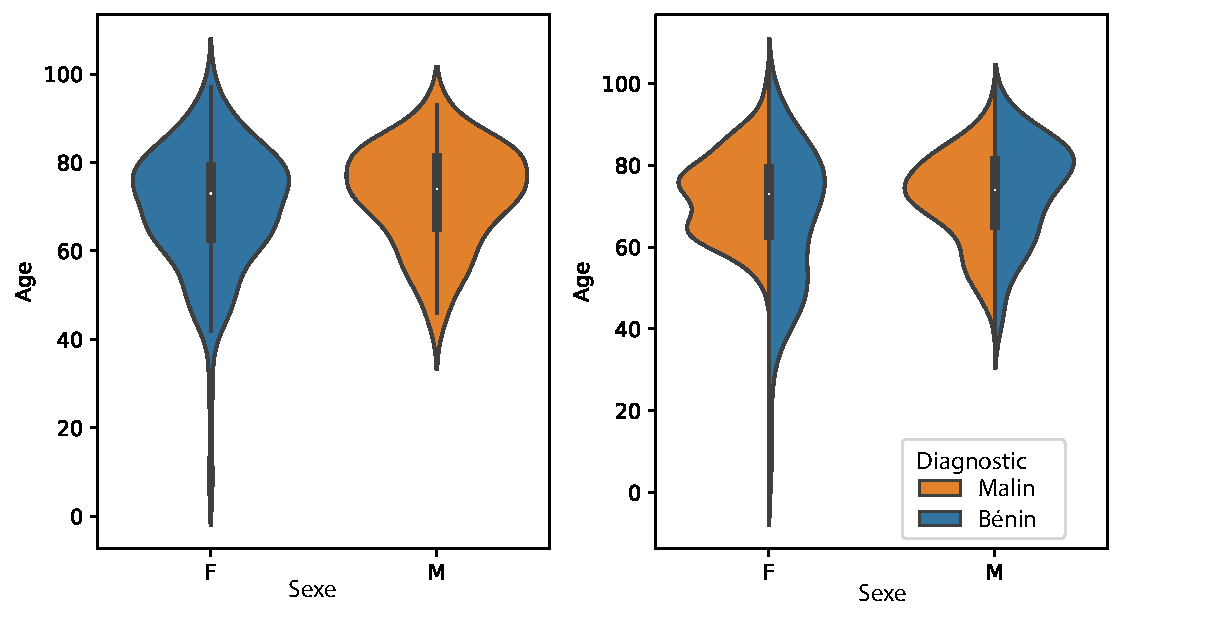
\includegraphics[width=0.8\linewidth]{contents/chapter_3_1/resources/statistics_age_sex.pdf}
    \caption{A gauche, répartition en fonction de l'âge et du sexe. A droite, répartition entre l'âge et le sexe en tenant compte du diagnostic binaire.}
    \label{fig:statistics_age_sex}
\end{figure}\par

Les acquisitions ont été à chaque fois réalisées par l'un des 3 experts investigateurs de l'étude clinique~\cite{Cinotti2018}. Tout cas de collisions de tumeurs au sein d'un même groupe a été exclu de cette étude. En ce qui concerne la modalité de dermatoscopie, les données ont été produites à l'aide d'une caméra PowerShot® G7~\textsuperscript{\ref{footnote:device_powershot}} couplée au dispositif proposé par Fotofinder~\textsuperscript{\ref{footnote:device_fotofinder}}. Pour ce qui est de la modalité de \gls{rcm}, les données proviennent d'un VivaScope 3000®~\textsuperscript{\ref{footnote:device_mavig}}. En revanche, aucune information liée à l'acquisition des données de photographie clinique n'a été mentionnée.\par

L'intérêt de ces trois modalités est grand dans le contexte de la dermatologie puisqu'elles représentent le processus \textit{classique} de prise en charge clinique, de la modalité la moins onéreuse avec la \textbf{photographie clinique} mais également la moins précise, à des modalités plus onéreuses, également plus riche en information, avec la \textbf{\gls{rcm}}. Ainsi, chaque modalité permet au praticien de réduire la zone d'incertitude chez un patient souffrant d'une pathologie de la peau.

\addtocounter{footnote}{1}
\footnotetext[\thefootnote]{Source~: Canon Powershot®, Canon, Tokyo, Japon. \label{footnote:device_powershot}}
\addtocounter{footnote}{1}
\footnotetext[\thefootnote]{Source~: FotoFinder Systems GmbH, Bad Birnbach, Allemagne. \label{footnote:device_fotofinder}}
\addtocounter{footnote}{1}
\footnotetext[\thefootnote]{Source~: Distribué en Europe par MAVIG GmbH, Munich, Allemagne. \label{footnote:device_mavig}}

Afin d'évaluer les performances de praticiens face à ces lésions, les investigateurs ont eu recours à 21 dermatologues détenant une expertise des modalités d'imagerie non-invasives. Ces experts sont répartis de manière homogène selon leurs compétences respectives pour chacun des dispositifs. Ainsi, le panel d'évaluation se décompose de la façon suivante~: 
\begin{inlinerate}
    \item 6 experts sont soumis à l'ensemble des modalités,
    \item 15 experts sont soumis à l'évaluation de la photographie clinique et de la dermatoscopie (dont 9 uniquement dédiés a ces deux modalités),
    \item et 12 sont soumis à la \gls{rcm} (dont 6 uniquement dédiés à la \gls{rcm})~\cite{Cinotti2018}.
\end{inlinerate}
La répartition de ces experts est résumée en \Cref{fig:experts_evaluation}.\par

\begin{figure}[H]
    \centering
    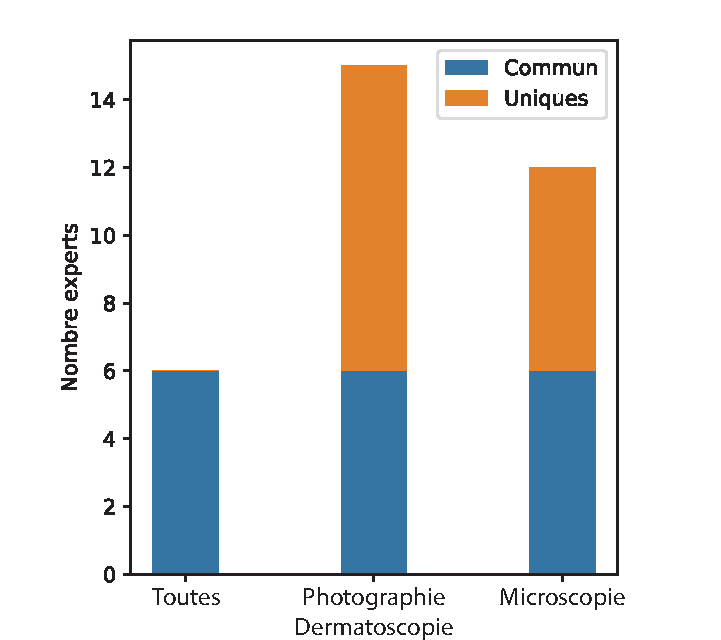
\includegraphics[width=0.6\linewidth]{contents/chapter_3_1/resources/experts_evaluation.pdf}
    \caption{Répartition du panel de 21 dermatologues sur l'évaluation des diverses modalités~\cite{Cinotti2018}.}
    \label{fig:experts_evaluation}
\end{figure}\par

Ces experts ont évalué la gravité pour chaque cas clinique présenté selon les termes bénin et malin. Afin d'éviter un biais de la part des experts qui ont réalisé l'évaluation sur les 3 modalités, ceux-ci ont été sollicités sur trois journées différentes~: 
\begin{inlinerate}
    \item une première journée d'évaluation ne comprenant que les images de photographie clinique et de dermatoscopie,
    \item une seconde journée d'évaluation ne comprenant que les images de \gls{rcm},
    \item et une dernière journée d'évaluation sur l'ensemble de la base d'images.
\end{inlinerate}
Par ailleurs, les cas cliniques ont été présentés dans un ordre différent entre chaque journée d'évaluation afin d'éviter des biais liés à l'activité précédente des experts.\par

La base d'images utilisée pour cette évaluation nous été remise, et ses données sensibles ont été anonymisées afin de ne pas pouvoir ré-identifier les patients. La structure de cette base peut être appréhendée sur la \Cref{fig:db_structure} - Gauche, et se compose~:
\begin{itemize}
    \item d'un \textbf{tableau de lésions}, sous forme de fichier \gls{csv} et contenant~:
    \begin{itemize}
        \item \textbf{en colonne}, les diverses informations relatives au patient, soit \textit{l'âge, le sexe, la zone, son diagnostic binaire issu de l'histologie (malin ou bénin) et diagnostic précis},
        \item \textbf{en ligne}, les divers enregistrements liés à chaque lésion respectant les champs précisé en colonne.
    \end{itemize}
    \item d'un \textbf{répertoire d'images} comprenant les divers cas clinique recensés dans l'étude sous divers formats image.
\end{itemize}\par

Afin d'exploiter au mieux cette base, quelques modifications ont été apportées. D'une part, la diversité des formats images est un frein quant à la gestion de ces données et nous avons opté pour un format matriciel sans perte de type bitmap. D'autre part, la structure de la base dans l'état ne permettait pas l'utilisation d'annotations au niveau des images ou supplémentaires à d'autres niveaux. Afin de rendre plus dynamique cette partie, nous avons opté pour une structure reprenant le tableau des lésions initial, lié à des répertoires associés à chaque lésion. Ce procédé est ainsi répété de manière récursive, chaque dossier de lésion se compose lui même de tableaux d'annotations propre au type d'annotations stockées. Par ailleurs, certains apports d'informations ont été réalisés pour permettre un bon déroulement de la suite de notre travail, tel que l'appartenance à un patient afin de ne pas proposer des données d'un même patient lors de l'entraînement et du test. La \Cref{fig:db_structure} - Droite synthétise la structure de cette base après modification.\par

\begin{figure}[H]
\centering
    \begin{subfigure}{.45\textwidth}
      \centering
      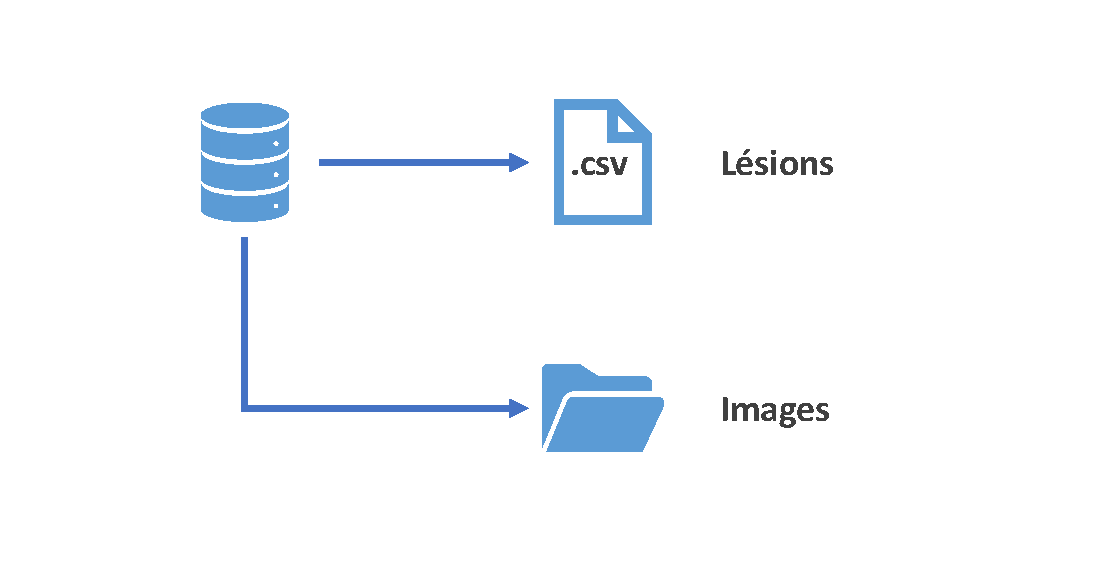
\includegraphics[width=\linewidth]{contents/chapter_3_1/resources/scheme_dbstructure_old.pdf}
    \end{subfigure}
    \begin{subfigure}{.45\textwidth}
      \centering
      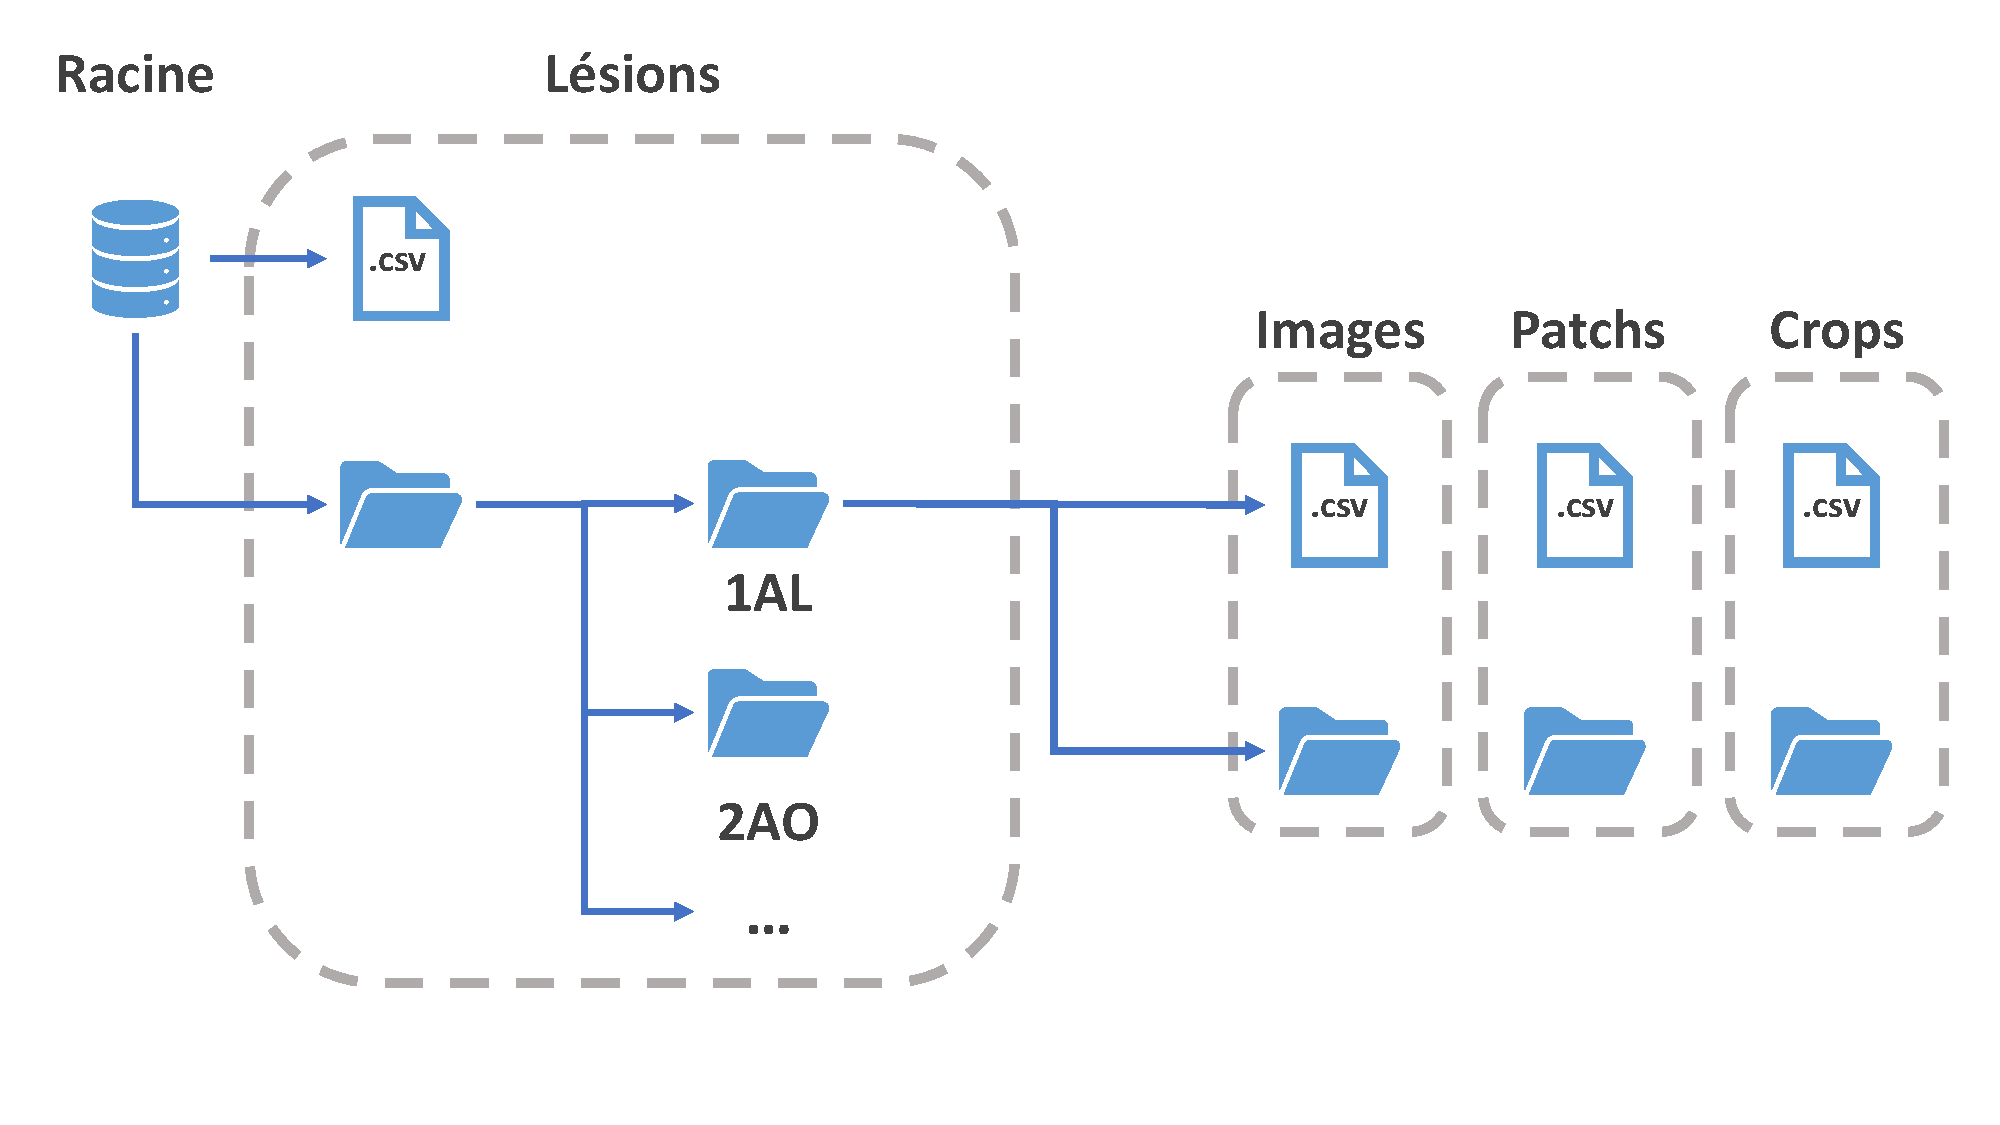
\includegraphics[width=\linewidth]{contents/chapter_3_1/resources/scheme_dbstructure_new.pdf}
    \end{subfigure}
    \caption{Schéma de l'organisation de la base de ressources employée. A gauche, la base initiale et à droite, la base restructurée afin de supporter de nouvelles annotations.}
    \label{fig:db_structure}
\end{figure}\par

\section{Méthodes clinique}
\label{sec:clinical_methods}
Pour permettre l'identification de pathologie en dermatologie plus routinière, la mise en avant de critères de diagnostic est une démarche clé permettant de rendre cette tâche plus efficace. Cette mise en avant de critères à été débutée au milieu des années 1980, sous la forme:
\begin{itemize}
    \item d'\textbf{acronyme}: l'idée est de proposer une méthode de diagnostic facile à mémoriser. Le travail de Friedman est un exemple, bien que révisé, le critère ABCD(E) est encore utilisé et applicable par de nombreuses personnes expertes ou non~\cite{Friedman1985}.
    \item de \textbf{liste}: de critères positifs et négatifs, correspondant à des caractéristiques rédhibitoires ou non, et amenant à un score final. Ce score variera selon la pathologie considérée et permettra d'en déduire une décision à prendre. L'un des exemple dans le cadre de lésions pigmentées est celui de MacKie en 1986~\cite{mackie1986}. Ces critères ont été révisés et se destinent néanmoins à un public expert. 
\end{itemize}\par

Ces démarches \textit{algorithmiques} de diagnostic, ainsi nommées, se sont progressivement étendues à d'autre pathologies et dispositifs d'analyse médicaux. Ils permettent de se référer à des critères essentiels en cas de doute. Le \gls{rcm} n'est pas exempt de ces démarches simplifiées, notamment pour le diagnostic du \gls{lm} avec les travaux de Pellacani et Guitera~\cite{Pellacani2007, Guitera2010}. Ces deux travaux proposent sous forme de table de critères ceux jugés positifs et négatifs, dont la \Cref{tab:rcm_algorithm_lentigo} donne un aperçu de la production de ces articles. Leur étude comptabilise 81 cas de \gls{lm} et 203 lésions bénignes, sur lesquels un seuil de score de 2 a été jugé comme pertinent au regard de l'étude statistique menée. Celui-ci a permis de détecter avec 85\% de sensibilité et 76\% de spécificité les \gls{lm}.\par

\begin{table}[H]
\centering
    \begin{tabular}{ll}
        \toprule
        Type de caractéristiques                        & Caractéristiques                                              \\\hline
        \multirow{2}{*}{Positives Majeures (+2 points)} & Papilles à contour faiblement définis                         \\\cline{2-2}
                                                        & Cellules pagétoides rondes >\SI{20}{\micro\metre}             \\\hline
        \multirow{3}{*}{Positives Mineures (+1 points)} & Présence de cellules atypiques dans la \gls{dej}              \\\cline{2-2}
                                                        & Combinaison de follicule / cellules atypique / pagétoide      \\\cline{2-2}
                                                        & Présence de cellules nucléées au sein de papilles              \\\hline
        Négatives Mineures (-1 points)                  & Motif en alvéoles larges                                      \\
        \bottomrule
    \end{tabular}
\caption{Caractéristiques observables par \gls{rcm} jugées pertinentes pour la détection du \gls{lm}~\cite{Guitera2010}.}
\label{tab:rcm_algorithm_lentigo}
\end{table}\par
 
Ainsi, une caractéristique a été déterminée comme pertinente par leurs auteurs~\cite{Pellacani2007, Guitera2010} lorsque celle-ci s'exprimait de manière plus significative dans l'un des deux groupes pathologiques (\gls{lm} ou bénin). L'un de ces travaux~\cite{Guitera2010} procède à une analyse de ces caractéristiques par profondeur croissante de la peau, dont nous listons quelques uns des éléments majeurs~:
\begin{itemize}
    \item au niveau de \textbf{l'épiderme}, les auteurs ont constaté que les pathologies de \gls{lm} comportent un désordre des cellules de l'épiderme (56\% des lésions \gls{lm} contre 18\% des lésions bénignes). Également, une infiltration pagétoïde a été reportée dans la plupart des cas de \gls{lm} (75\% des lésions \gls{lm} contre 28\% des lésions bénignes). En opposition, un épiderme homogène, caractérisé par des motifs en nids d'abeille, ont été constatés dans 92\% des cas bénins. Ces éléments peuvent être observées sur la \Cref{fig:example_rcm_pattern_1}.
    \item au niveau de la \textbf{\gls{dej}}, les auteurs ont constaté que les papilles non démarquées étaient observées dans la majorité des \gls{lm} (68\% \gls{lm} and in 17\% des cas bénins). Ces éléments peuvent être observées sur la  \Cref{fig:example_rcm_pattern_2}.
    \item au niveau du \textbf{derme}, 15\% des cas de \gls{lm} présentent des cellules nucléées large contre 2\% des lésions bénignes. Ces élements peuvent être observées sur la \Cref{fig:example_rcm_pattern_3}.
\end{itemize}\par

\begin{figure}[H]
    \begin{center}
        \includegraphics[width=0.9\linewidth]{contents/chapter_3_1/resources/example_rcm_pattern_1.pdf}
        \caption{Cas de données cliniques \gls{rcm} en provenance de l'épiderme par Guitera~\cite{Guitera2010}. En a) et b), exemples de motifs en large nids d'abeille (\textit{broadened honeycomb pattern}), respectivement d'un kératose séborrhéique et de peau normale ; en c), exemples de motifs de pavés atypiques (\textit{atypical cobblestone pattern}) issus d'un \gls{lm} ; en d), exemples de \textit{large pagetoid} cellules propre au \gls{lmm}. Repère~: barre = \SI{50}{\micro\metre}.}
        \label{fig:example_rcm_pattern_1}
    \end{center} 
\end{figure}\par

\begin{figure}[H]
    \begin{center}
        \includegraphics[width=0.7\linewidth]{contents/chapter_3_1/resources/example_rcm_pattern_2.pdf}
        \caption{Cas de données cliniques \gls{rcm} par Guitera~\cite{Guitera2010}. En a) et au niveau de la flèche, exemple de papille à frontière non marqué (\textit{Nonedge papillae}) et de cellules atypique d'un \gls{lm} acquise à la jonction \gls{dej} ; En b), exemple de papilles à frontières marquées (\textit{Edge papillae}) d'une pathologie bénigne. En c), exemple de cellules atypiques au niveau de la \gls{dej} typique de \gls{lm} ; En d), exemple de halo noir autour de cellules atypiques de l'épiderme issue d'un \gls{lm}. Repère~: barre = \SI{50}{\micro\metre}.}
        \label{fig:example_rcm_pattern_2}
    \end{center} 
\end{figure}\par

\begin{figure}[H]
    \begin{center}
        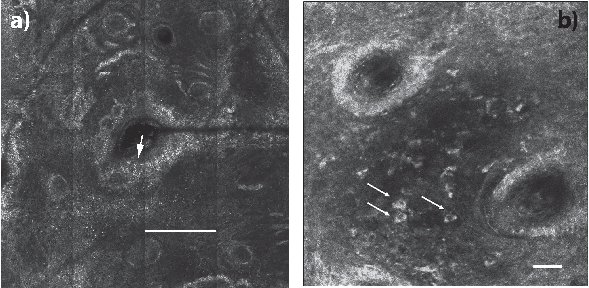
\includegraphics[width=0.8 \linewidth]{contents/chapter_3_1/resources/example_rcm_pattern_3.pdf}
        \caption{Cas de données cliniques \gls{rcm} par Guitera~\cite{Guitera2010}. En a), exemple de cellules atypiques à proximité d'un follicule pileux au sein de la \gls{dej} sur un \gls{lm} ; En b), exemple de cellules nucléés du derme d'un \gls{lm}. Repère~: barre = \SI{50}{\micro\metre}.}
        \label{fig:example_rcm_pattern_3}
    \end{center} 
\end{figure}\par

Dans l'étude menée par Cinotti et al.~\cite{Cinotti2018}, les auteurs investigateurs ont demandé d'évaluer certaines caractéristiques récurrentes de la littérature, parmi lesquelles~:
\begin{itemize}
    \item la présence de grandes cellules pagétoïdes arrondies, présentes dans 37\% des \gls{lm} et seulement 5\% des pathologies bénignes,
    \item la présence de grandes cellules dendritiques dans l'épiderme, présentes dans 81\% des \gls{lm} contre 13\% des pathologies bénignes,
    \item la localisation au niveau des follicules pileux des cellules atypiques, dans 62\% des \gls{lm} et seulement 7\% des pathologies bénignes.
\end{itemize}\par


Par ailleurs, cette étude est conforme aux recommandations de la déclaration de Helsinky et le protocole de cette étude soumis à l'agrément du \gls{chu} de Saint-Étienne pour l'exploitation de ces données cliniques (Comité d'examen institutionnel numéro 672016 / CHUSTE).



\section{Démarches d'aide au diagnostic}
\label{sec:cad_methods}

\cite{Wiltgen2008}
\cite{Halimi2017a}



